\documentclass[xcolor={usenames,dvipsnames}, 
	hyperref={
	colorlinks=true, 						% Internetseiten werden farblich hervorgehoben
	linkcolor=black, 						% Farbe für interne Referenzen
	urlcolor=black,							% Farbe für Links auf Webseiten
	citecolor=black,						% Farbe für Zitate \cite{<bibtexid>}
	pdfpagelabels=false,
	%pdfauthor={}, 
	%pdftitle={}				% Verewigt Author und Titel in PDF-Informationen
	},
	ignorenonframetext,			% Keine Nummerierung auf erster Folie
	compress					% Minimize navigation bars
]{beamer}
%===== Formatierungs-Packages =====
	\usepackage[T1]{fontenc}				% fontenc und inputenc ermöglichen
	%\usepackage[latin1]{inputenc}			% Silbentrennung und Eingabe 
	\usepackage[utf8]{inputenc}
	\usepackage{lmodern}					% Schrift wirkt (in pdf-Ausgabe) fließender
  							
%===== Sprach-Packages =====
	\usepackage[ngerman]{babel}			% Babel für diverse Sprachanpassungen, 
  										% z.B. Anführungszeichen
%===== Interne Latex-Packages =====
	\usepackage{fixltx2e} 				% Verbessert einige Kernkompetenzen von LaTeX2e
  
%===== Mathe-Packages ======
	\usepackage{amsmath, amssymb, amsfonts} 	% Mathematische Features der American Mathematical
	\usepackage{cancel}
	\usepackage[output-decimal-marker={,},  	% Deutsche Dezimaltrennung mit Komma
		separate-uncertainty = true,		  	% Fehlerangabe: \SI{3(2)}{\tesla}
		per-mode=fraction,					  	% Einheiten als Bruch darstellen
		exponent-product = \cdot,			  	% Exponentialschreibweise mit Malzeichen \SI{3e8}{\tesla}
		math-ohm,
		range-phrase = -					% Option für Bereichsangabe \SIrange{3}{4}{\tesla}
		]{siunitx} 						  	
 								% Elementar wichtig für Einheiten \siunit{3}{\milli\meter}					% \unit{\tesla}, \num{<Zahl>}
  
%===== Grafik/Tabellen-Packages ======
	\usepackage{xcolor}						% Erlaubt das Verwenden von Farben
	\usepackage{graphicx} 					% Erlaub das Einbinden von Bildern
	\usepackage{multirow} 					% Erlaubt multicolumn{3}{c}{Bla}
	\usepackage{rotating} 					% Erlaub sidewaystable-Umgebung
	%\usepackage[miktex,subfolder,siunitx]{gnuplottex} % Gnuplot in Latex
  
%===== bibliography =====
	\usepackage[numbers,square]{natbib} 	%Einbinden der Bibliothek mit "[1]" Zitat
  
%===== Sonstiges ======
\usepackage{subfigure} 
\usepackage[labelformat=empty]{caption}   % Keine Abbildung... bei Bildunterschrift
	\usepackage{url}						% Erlaubt das Einbinden einer URL
	\usepackage{pdfpages}					% \includepdf{<file>.pdf} wird verfügbar
	\usepackage[flushmargin,				% Fußnoten bündig mit Seitenrändern
		hang,									% Hängender Zeilenumbruch bei Fußnoten 
		bottom]{footmisc}						% Zwingt Fußnoten ans Ende der Seite
	\usepackage{hyperref} 	% Hyperref-Package verlinkt interne Referenzen
	\usepackage{lipsum} 	% Für Testzecke \lipsum[1]
	
%===== Back-Up Seiten ======	
    \newcommand{\backupbegin}{
   \newcounter{finalframe}
   \setcounter{finalframe}{\value{framenumber}}
}
    \newcommand{\backupend}{
   \setcounter{framenumber}{\value{finalframe}}
}
  
%===== Beamer template - Spezifikationen ======
	\usepackage{beamerthemetexsx}
	\setbeamertemplate{mini frames}[box]
	%\renewcommand{\bibsection}{\section{Literature}}

%===== Listing code ======
\usepackage{listings}
\usepackage{color}

%from https://stackoverflow.com/questions/3175105/writing-code-in-latex-document
\definecolor{dkgreen}{rgb}{0,0.6,0}
\definecolor{gray}{rgb}{0.5,0.5,0.5}
\definecolor{mauve}{rgb}{0.58,0,0.82}

\lstset{frame=tb,
  language=Java,
  aboveskip=3mm,
  belowskip=3mm,
  showstringspaces=false,
  columns=flexible,
  basicstyle={\small\ttfamily},
  numbers=none,
  numberstyle=\tiny\color{gray},
  keywordstyle=\color{blue},
  commentstyle=\color{dkgreen},
  stringstyle=\color{mauve},
  breaklines=true,
  breakatwhitespace=true,
  tabsize=3
}

%==== Informationen ====
	
	\title[Clustering]{Clustering} 
	%\subtitle[Optionaler Subtitle]{Optionaler Subtitle des sehr langen Titels der Präsentation}
	\author{Manuel Mauch, Marius Köppel}
	\institute[DM 17/18]{DM 17/18}
	\date{12.\,12.\,2017}
	%Titelgraphic
	%\includegraphics[keepaspectratio]{TopPDF.jpeg}
	%\titlegraphic{\includegraphics[height=2.1cm,keepaspectratio]{TopPDF.jpeg}}
	%Logo on each slide
	%\logo{
		%\vspace*{-.25cm} %vertical displacement of logo position
		%
\includegraphics[height=1cm,keepaspectratio]{Logos/Gefoerdert_vom_BMBF_eng.jpg}
		%\hspace*{.25cm} %horizontal displacement of logo position
		%}
	%}
%\pdfminorversion=4	% PDF 1.4, um Lesefehlern mit Acrobat entgegenzuwirken
	
%==== Begin presentation ====

\begin{document}

\begin{frame}[plain,noframenumbering]  %Keine Fußzeile auf erster Seite und keine Nummerierung
	\titlepage
\end{frame}
	
\addtocounter{framenumber}{-1} %Titelseite wird nicht gezählt im Counter

%\setbeamertemplate{footline}{authorinstitutetitle} %Aktiviere Fußzeile

%---------------------------------------------------------------------

\begin{frame}
	\frametitle{Inhaltsverzeichnis}
	\tableofcontents
\end{frame}%[pausesections]} 

%---------------------------------------------------------------------

\section{Agglomerative and Divisive Clustering}
\begin{frame}
   \frametitle{Agglomerative and Divisive Clustering}
   The goal of this task was to create three dentograms for each dataset with R and the provided algorithmus Agnes and Diana. First we will present this algorithmus and then we will discuss the dentograms of each dataset.
\end{frame}

\begin{frame}
   \frametitle{Agnes}

    \begin{itemize}
        \item Blabal
        \item Blabal
    \end{itemize}

\end{frame}

\begin{frame}
   \frametitle{Diana}

    \begin{itemize}
        \item Blabal
        \item Blabal
    \end{itemize}

\end{frame}

\begin{frame}
   \frametitle{S2 from S-sets}

For this dataset we were not able to create to plots, because it took to much time for proceed.

\end{frame}

\begin{frame}
   \frametitle{Seeds}
\begin{figure}[ht!]
\caption{Detaset Seeds}
\centering
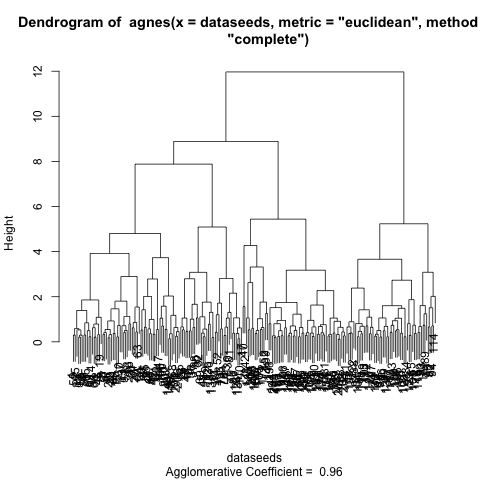
\includegraphics[width=0.7\textwidth]{plots/ang1dataseeds.png}
\end{figure}
\end{frame}

\begin{frame}
   \frametitle{Seeds}
\begin{figure}[ht!]
\caption{Detaset Seeds}
\centering
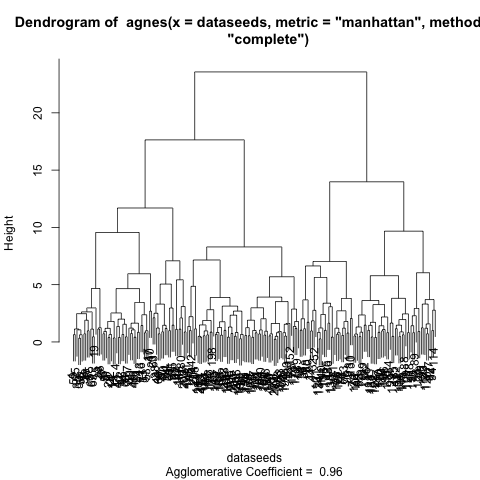
\includegraphics[width=1\textwidth]{plots/ang2dataseeds.png}
\end{figure}
\end{frame}

\begin{frame}
   \frametitle{Seeds}
\begin{figure}[ht!]
\caption{Detaset Seeds}
\centering
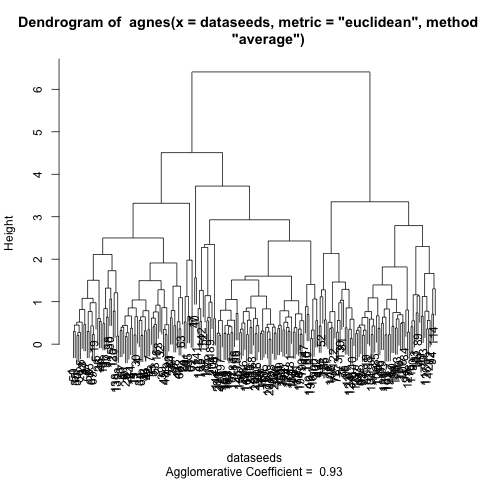
\includegraphics[width=1\textwidth]{plots/ang3dataseeds.png}
\end{figure}
\end{frame}

\begin{frame}
   \frametitle{Seeds}
\begin{figure}[ht!]
\caption{Detaset Seeds}
\centering
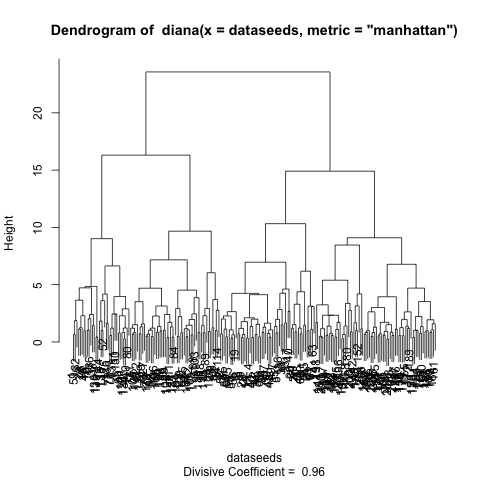
\includegraphics[width=1\textwidth]{plots/dv1dataseeds.png}
\end{figure}
\end{frame}

\begin{frame}
   \frametitle{Seeds}
\begin{figure}[ht!]
\caption{Detaset Seeds}
\centering
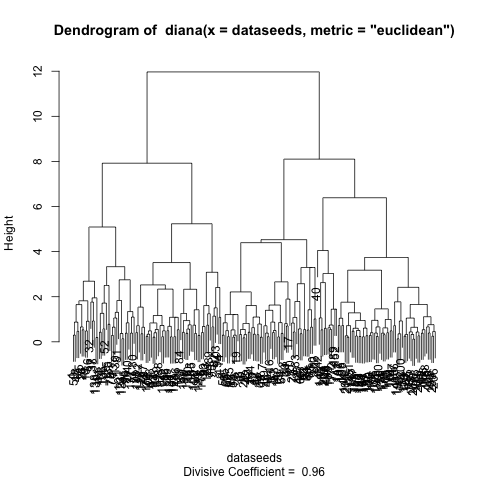
\includegraphics[width=1\textwidth]{plots/dv2dataseeds.png}
\end{figure}
\end{frame}

\begin{frame}
   \frametitle{Dim032 from DIM-sets (high)}
\begin{figure}[ht!]
\caption{Detaset Dim032}
\centering
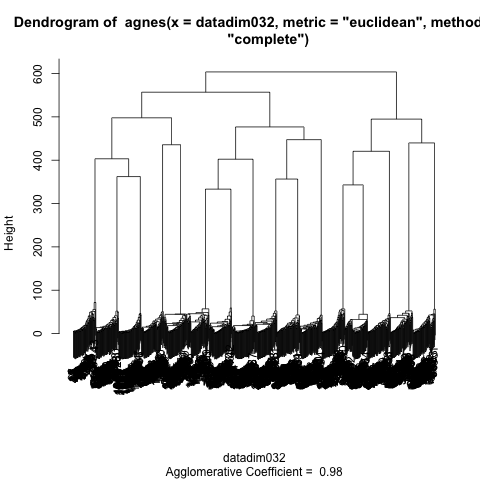
\includegraphics[width=1\textwidth]{plots/ang1dim032.png}
\end{figure}
\end{frame}

\begin{frame}
   \frametitle{Dim032 from DIM-sets (high)}
\begin{figure}[ht!]
\caption{Detaset Dim032}
\centering
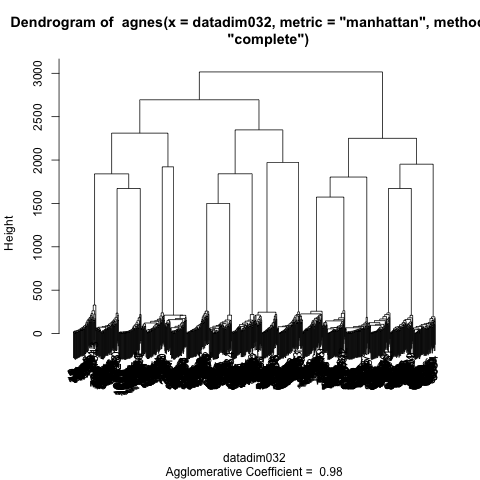
\includegraphics[width=1\textwidth]{plots/ang2dim032.png}
\end{figure}
\end{frame}

\begin{frame}
   \frametitle{Dim032 from DIM-sets (high)}
\begin{figure}[ht!]
\caption{Detaset Dim032}
\centering
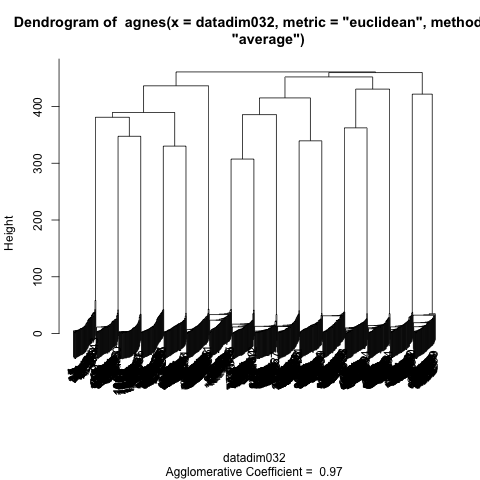
\includegraphics[width=1\textwidth]{plots/ang3dim032.png}
\end{figure}
\end{frame}

\begin{frame}
   \frametitle{Dim032 from DIM-sets (high)}
\begin{figure}[ht!]
\caption{Detaset Dim032}
\centering
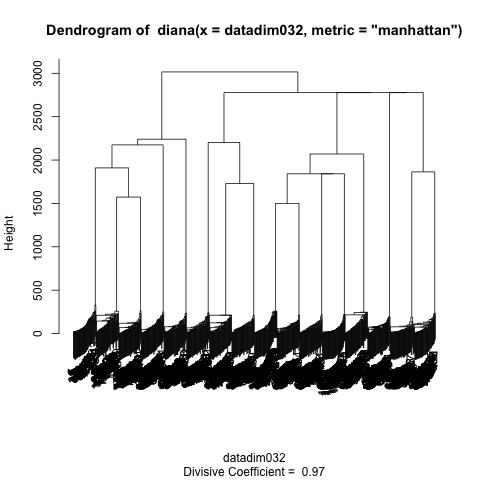
\includegraphics[width=1\textwidth]{plots/dv1dim032.png}
\end{figure}
\end{frame}

\begin{frame}
   \frametitle{Dim032 from DIM-sets (high)}
\begin{figure}[ht!]
\caption{Detaset Dim032}
\centering
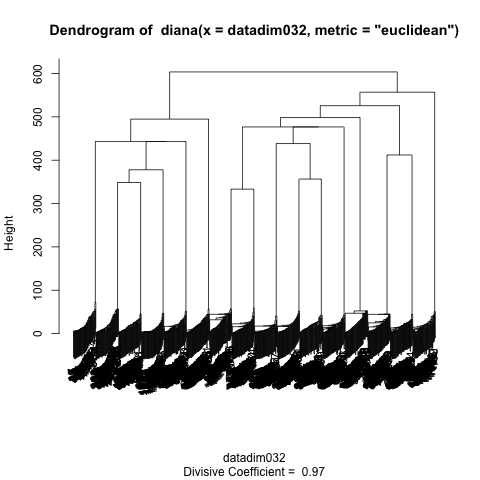
\includegraphics[width=1\textwidth]{plots/dv2dim032.png}
\end{figure}
\end{frame}

\begin{frame}
   \frametitle{Conclusion}
TODO (MANUEL): Was ist hight in dentogram?, Wie gehen die Algorithmen und Interpretation der unterschiedlichen Teile.
\end{frame}


%---------------------------------------------------------------------

\section{K-means}
\begin{frame}
   \frametitle{K-means}
\lstinputlisting[language=Python]{k_mean1.py}
\end{frame}

\begin{frame}
   \frametitle{K-means}
\lstinputlisting[language=Python]{k_mean2.py}
\end{frame}

\begin{frame}
   \frametitle{K-means}
\lstinputlisting[language=Python]{k_mean3.py}
\end{frame}

\begin{frame}
   \frametitle{K-means}
\lstinputlisting[language=Python]{k_mean4.py}
\end{frame}

\begin{frame}
   \frametitle{K-means}
\lstinputlisting[language=Python]{k_mean5.py}
\end{frame}

\begin{frame}
   \frametitle{K-means}
\lstinputlisting[language=Python]{k_mean6.py}
\end{frame}

\begin{frame}
   \frametitle{K-means}
\lstinputlisting[language=Python]{k_mean7.py}
\end{frame}

\begin{frame}
   \frametitle{K-means}
\begin{center}
  \begin{tabular}{ c | c | c | c }
    Data & RAND & norm. mutual info. & purity of clusters \\ 
    \hline
    jain.txt & 2 & 6 & 1 \\
    compound.txt & 3 & 3 & 1 \\
  \end{tabular}
\end{center}
Set S2 had no lable so it was not possible to calculate the best k
\end{frame}

\begin{frame}
   \frametitle{K-means}
\begin{figure}[ht!]
\caption{True Clusters}
\centering
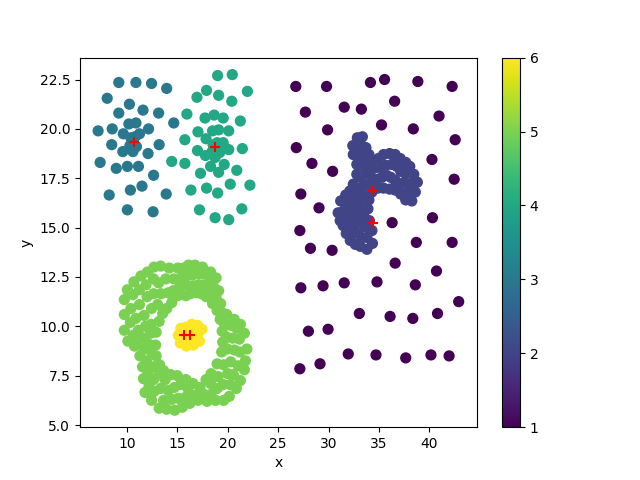
\includegraphics[width=0.8\textwidth]{plots/k_mean_0.png}
\end{figure}
\end{frame}

\begin{frame}
   \frametitle{K-means}
\begin{figure}[ht!]
\caption{k = 1}
\centering
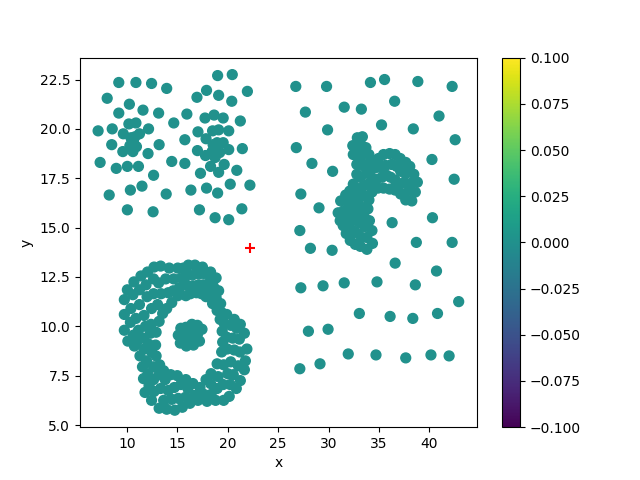
\includegraphics[width=0.8\textwidth]{plots/k_mean_1.png}
\end{figure}
\end{frame}

\begin{frame}
   \frametitle{K-means}
\begin{figure}[ht!]
\caption{k = 2}
\centering
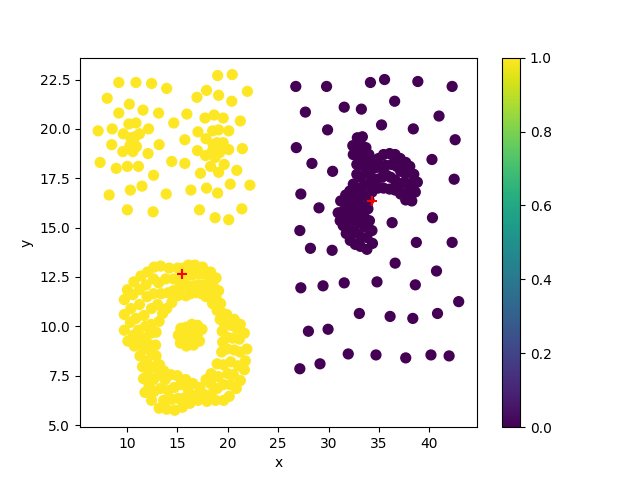
\includegraphics[width=0.8\textwidth]{plots/k_mean_2.png}
\end{figure}
\end{frame}

\begin{frame}
   \frametitle{K-means}
\begin{figure}[ht!]
\caption{k = 3}
\centering
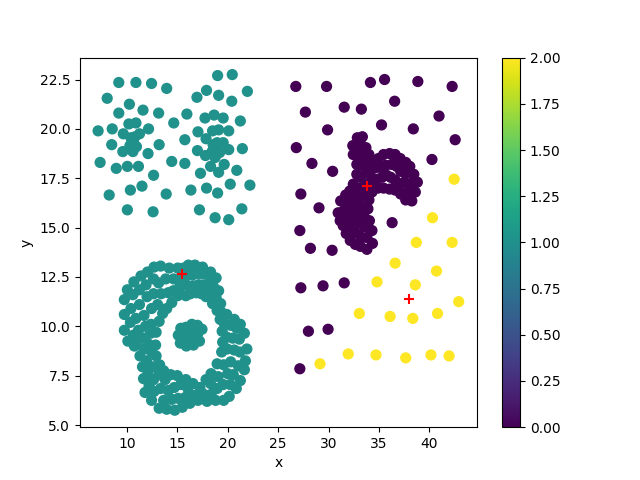
\includegraphics[width=0.8\textwidth]{plots/k_mean_3.png}
\end{figure}
\end{frame}

\begin{frame}
   \frametitle{K-means}
\begin{figure}[ht!]
\caption{k = 3}
\centering
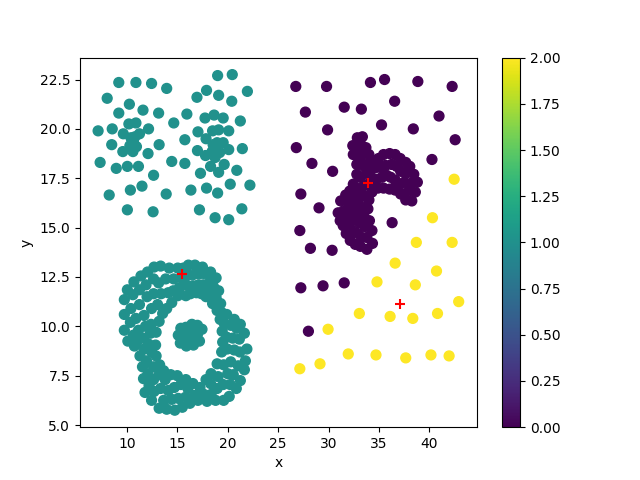
\includegraphics[width=0.8\textwidth]{plots/k_mean_4.png}
\end{figure}
\end{frame}

\begin{frame}
   \frametitle{K-means}
\begin{figure}[ht!]
\caption{k = 3}
\centering
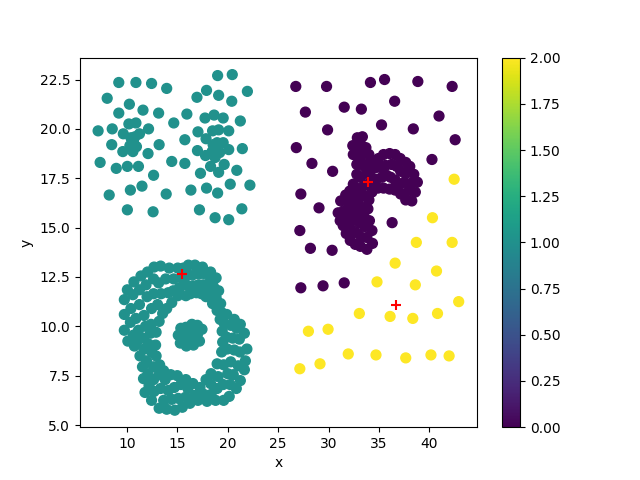
\includegraphics[width=0.8\textwidth]{plots/k_mean_5.png}
\end{figure}
\end{frame}

\begin{frame}
   \frametitle{K-means}
\begin{figure}[ht!]
\caption{k = 3}
\centering
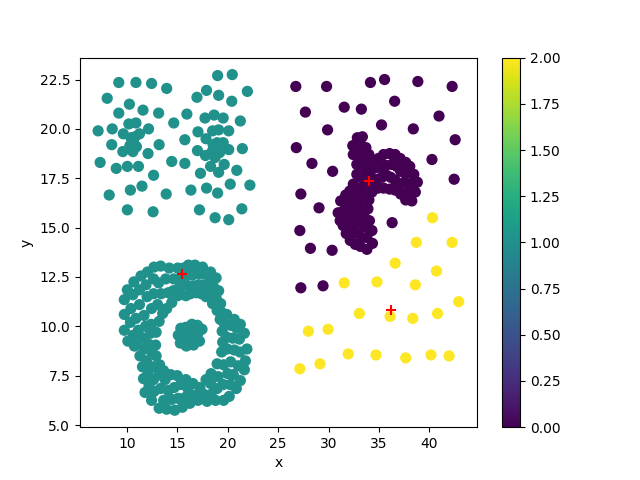
\includegraphics[width=0.8\textwidth]{plots/k_mean_6.png}
\end{figure}
\end{frame}

\begin{frame}
   \frametitle{K-means}
\begin{figure}[ht!]
\caption{k = 3}
\centering
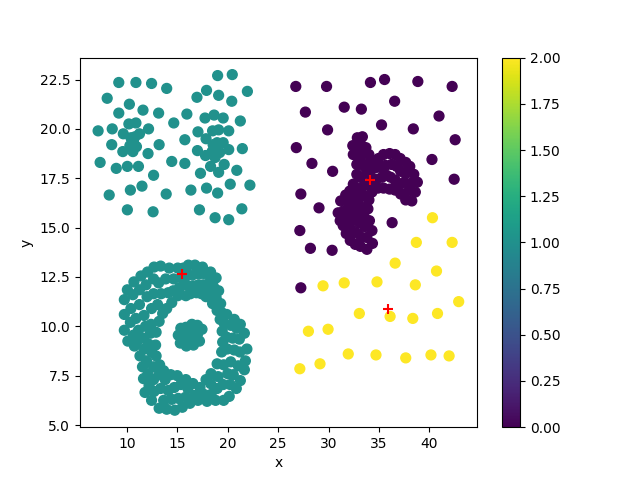
\includegraphics[width=0.8\textwidth]{plots/k_mean_7.png}
\end{figure}
\end{frame}

\begin{frame}
   \frametitle{K-means}
\begin{figure}[ht!]
\caption{k = 4}
\centering
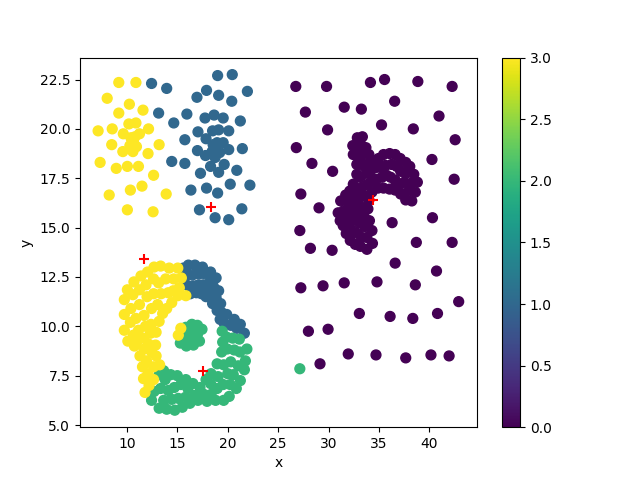
\includegraphics[width=0.8\textwidth]{plots/k_mean_8.png}
\end{figure}
\end{frame}

\begin{frame}
   \frametitle{K-means}
\begin{figure}[ht!]
\caption{k = 4}
\centering
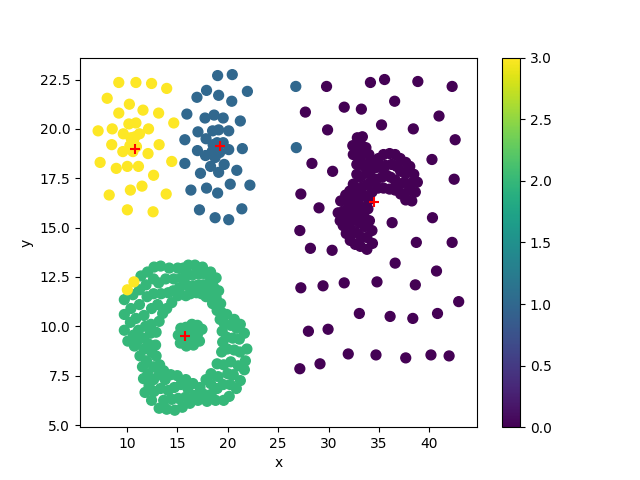
\includegraphics[width=0.8\textwidth]{plots/k_mean_9.png}
\end{figure}
\end{frame}

\begin{frame}
   \frametitle{K-means}
\begin{figure}[ht!]
\caption{k = 5}
\centering
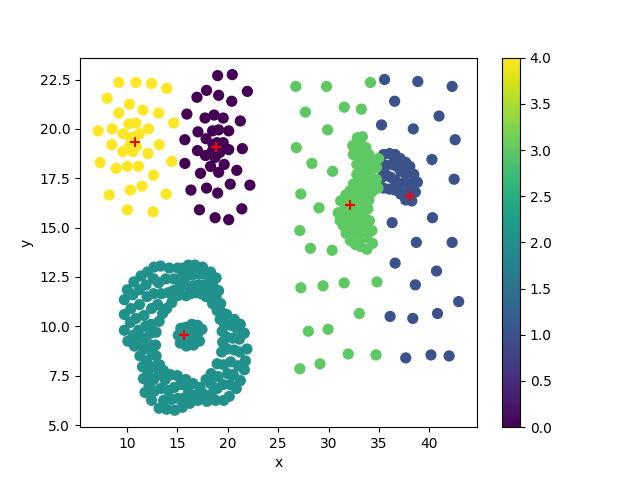
\includegraphics[width=0.8\textwidth]{plots/k_mean_10.png}
\end{figure}
\end{frame}

%---------------------------------------------------------------------

\section{EM}
\begin{frame}
   \frametitle{EM}
\lstinputlisting[language=Python]{log-1.py}
\end{frame}

\begin{frame}
   \frametitle{EM}
\lstinputlisting[language=Python]{log-7.py}
\lstinputlisting[language=Python]{log-6.py}
\end{frame}

\begin{frame}
   \frametitle{EM}
\lstinputlisting[language=Python]{log-5.py}
\end{frame}

\begin{frame}
   \frametitle{EM}
\lstinputlisting[language=Python]{log-2.py}
\end{frame}

\begin{frame}
   \frametitle{EM}
\lstinputlisting[language=Python]{log-4.py}
\end{frame}

\begin{frame}
   \frametitle{EM}
\lstinputlisting[language=Python]{log-3.py}
\end{frame}

\begin{frame}
   \frametitle{EM}
\begin{center}
  \begin{tabular}{ c | c | c | c }
    sig1 & sig2 & mu1 & mu2 \\ 
    \hline
    1.32 & 7.91 & 16.93 & 24.73 \\
  \end{tabular}
\end{center}
Value afer 20 steps: -1193.21
\end{frame}

\end{document}
    
%    \begin{figure}[hhh]
%    \begin{center}
%    \includegraphics[width=0.95\textwidth]{Top_Quark_Decay.jpeg}
%        \caption[bigbang]
%    \end{center}
%    \end{figure}

%\begin{columns}[T]
%    \begin{column}{.5\textwidth}
%    \begin{block}{Your textblock}
%    asfasfaf
%    \end{block}
%    \end{column}
%    \begin{column}{.5\textwidth}
%    \begin{block}{Your image}
%    %BILD
%    \includegraphics[width=.7\textwidth]{xx_tt_b.png}
%    \end{block}
%    \end{column}
%\end{columns}